\documentclass[11pt,a4paper]{article}
\usepackage{fontspec}
\usepackage{polyglossia}
\setdefaultlanguage{turkish}
\usepackage[margin=2.4cm]{geometry}
\usepackage{graphicx}
\usepackage{booktabs}
\usepackage{amsmath}
\usepackage[font=small,labelfont=bf]{caption}
\usepackage{xcolor}
\usepackage{microtype}
\usepackage[hidelinks]{hyperref}
\setlength{\emergencystretch}{3em}
\setlength{\parskip}{0.5em}
\setlength{\parindent}{0pt}
% LuaLaTeX ile derlenir (bu bilgisayarda XeLaTeX yok)
\newcommand{\kod}[1]{\texttt{#1}}
\newcommand{\olc}{\textsc{[Ölçüldü]}}
\newcommand{\yor}{\textsc{[Yorum]}}
\newcommand{\hip}{\textsc{[Hipotez]}}

\title{Merkezleme çalışmasının durumu: 17--18 Kasım 2026\\[0.3em]
\large Bulgular, yazılım değişiklikleri, açık işler ve nasıl devam edileceği}
\author{Hazırlayan: Claude (Anthropic)}
\date{20 Kasım 2026}

\begin{document}
\maketitle

\section*{Özet}

Bu rapor iki günlük çalışmayı toplar: 17 Kasım'da bobin kuadrupole sabitlendikten sonraki iki saatlik izleme
ölçümü (ayrıntısı \kod{raporlar/izleme\_2026-11-17/rapor.pdf}'te) ve 18 Kasım'da yazılımda yapılan değişiklikler
ile donanımda yapılan üç test. Başlıca sonuçlar:

\begin{enumerate}
\item \textbf{Kalibrasyon matrisi her gün yeniden kurulmak zorunda değil.} 6--17 Kasım'daki dokuz kalibrasyon,
kuadrupolün kendi eksenine göre döndürülünce tepeden tepeye en çok 5° farkla üst üste düşüyor \olc. Yazılım artık
kayıtlı bir kalibrasyonu seçip iki ölçümlük bir ``yön doğrulama'' ile kullanabiliyor.
\item \textbf{Enkoder artımlı; sıfırı her oturumda keyfi.} Bu yüzden arayüzde ``roll'' diye gösterilen açı
yerçekimine göre bir açı değildi \olc. Adını düzelttim. Yerçekimine göre gerçek skew için bir açı referansı
(ivmeölçer) gerekiyor; planı yazılı ama yapılmadı.
\item \textbf{Merkezleme 5 µm'ye inemiyordu çünkü 2 saniyelik tek ölçümün gürültüsü ~4 µm.} Ölçüm süresi 10
saniyeye çıkarılınca merkezleme yakınsadı: merkez $(2.5,\ -1.4)$~µm, 2 dakikada \olc.
\item \textbf{10 saniyelik ölçüm bir yan etki doğurdu.} 16:30'da sizin yaptığınız denemede ``okuma saati
sıçraması'' denetimi ölçümlerin yaklaşık yarısını reddetti ve üst üste üç ret motoru durdurdu \olc. Denetimin
eşiğini 0.6'dan 0.9'a çıkardım (Bölüm~\ref{sec:sicrama}). Bu değişiklik donanımda henüz denenmedi.
\item \textbf{Yeni arayüz hazır ama birleştirilmedi.} \kod{arayuz-duzen} dalında; gerçek ekranda ve donanımla
denenmedi (Bölüm~\ref{sec:durum}).
\end{enumerate}

\section{Nerede ne duruyor, nasıl devam edilir}
\label{sec:durum}

\textbf{Depo:} \kod{/home/selcuk/projeler/dipole-correction-at-quad}. Uzak depoya (GitHub) hiçbir şey
gönderilmedi; her şey yalnızca bu bilgisayarda.

\begin{table}[h]
\centering\small
\begin{tabular}{lp{9cm}}
\toprule
dal / etiket & ne var \\
\midrule
\kod{main} & 17--18 Kasım'ın tüm yazılım değişiklikleri (donanımda test edildi) ve sıçrama eşiği düzeltmesi
(\textbf{test edilmedi}). Şu an çalışma klasöründe bu dal açık. \\
\kod{arayuz-duzen} & Yeni arayüz düzeni (alt durum çubuğu, yeni sayfalar, Ayarlar sekmesi). \textbf{Birleştirilmedi,
donanımla denenmedi.} \\
\kod{merkezleme-18-kasim} & \kod{main}'in 18 Kasım öğleden sonrasındaki eski bir noktası (ara dal); silinebilir. \\
etiket \kod{lab-testi-oncesi-2026-11-18} & Donanım testlerinden önceki durum. \\
etiket \kod{merkezleme-2026-11-18-test} & Donanımda test edilmiş durum (10 s ölçüm, 8 yineleme). \\
\bottomrule
\end{tabular}
\caption{Git durumu. Bir şey ters giderse \kod{git checkout merkezleme-2026-11-18-test} ile donanımda denenmiş
duruma dönülür.}
\end{table}

\textbf{Çalıştırma:} \kod{./merkezle} gerçek donanımla (önce dönen bobin sekmesinde ``Başlat'' ile motor
çalıştırılır, sonra Merkezleme sekmesinde ``Merkezlemeyi başlat''), \kod{./merkezle kuru} güç kaynaklarına komut
göndermeden. Yeni arayüzü görmek için: \kod{git switch arayuz-duzen}. Beğenilirse: \kod{git switch main \&\&
git merge arayuz-duzen}.

\textbf{Testler:} \kod{python3 -m pytest -q tests} (\kod{main}'de 216, \kod{arayuz-duzen}'de 223 test) ve
\kod{donen\_bobin/host} içinde aynı komut (82 test). İkisi de geçiyor.

\textbf{Donanım test betikleri} (motor ve akım açarlar; her çalıştırmada kullanıcı onayı alınmalı):
\kod{python3 -m merkezleme.arayuz\_testi --kalibrasyon son --akimlardan --izleme-dk 10 --bekci} ve
\kod{python3 -m merkezleme.tani\_testi --akimlar-calistirma <klasör>}. Kayıtları \kod{kayitlar/} altına
yazarlar.

\textbf{Ne nerede:} \kod{README.md} (kullanım ve 18 Kasım değişiklikleri), \kod{planlar/YAPILACAKLAR.md} (açık işler),
\kod{planlar/yercekimi\_referansi\_PROMPT.md} (ivmeölçer takılınca yeni bir Claude oturumuna verilecek istem),
\kod{raporlar/} (raporlar ve analiz betikleri). Ham ölçüm kayıtları (\kod{kayitlar/}, \kod{calistirmalar/})
git'te yoktur; yalnızca bu bilgisayarda durur.

\section{Bulgular}

\subsection{Kalibrasyon matrisi günler arası aynı kalıyor}

Merkezleme, dört bobinin akımını küçük adımlarla değiştirip merkezin nasıl hareket ettiğini ölçerek bir matris
çıkarır (``kalibrasyon''; her sütun bir bobinin merkezi hangi yöne ve ne kadar ittiğidir). Her merkezlemenin başında
bu yedi dakikalık kalibrasyon yeniden yapılıyordu. Dokuz kalibrasyonu karşılaştırdım (Tablo~\ref{tab:matris},
Şekil~\ref{fig:matris}).

Ham sütun açıları günden güne çok değişiyor (örneğin I1 için $-146^\circ$, $+33^\circ$, $+128^\circ$, $-77^\circ$).
Ama her kalibrasyonda kuadrupol alanının kendi açısını, $\psi = \tfrac{1}{2}\arg C_2$, ölçebiliyoruz. Matrisin
sütunlarını bu açı kadar döndürünce dokuz matrisin hepsi aynı yere düşüyor: sütun açıları ortalama
$-46.8^\circ$, $+43.0^\circ$, $+134.3^\circ$, $-134.6^\circ$, her biri için tepeden tepeye en çok
$5.0^\circ$ yayılma \olc. Boyları da aynı: 9.5~A'de 2.0--2.4~µm/mA. 7~A'deki matrisin boyu daha büyük
(2.95--3.13~µm/mA), ama bu beklenen: merkezin mA başına kayması gradyenle ters orantılı ve
$2.2 \times 9.5/7 \approx 3.0$ \yor.

\begin{table}[h]
\centering\footnotesize
\begin{tabular}{lrrrrrrrrrl}
\toprule
kalibrasyon & A & $\psi$ & $\cos 2\psi$ & I1 ham & \multicolumn{4}{c}{kuadrupol çerçevesinde} & µm/mA & şüpheli \\
 & & (°) & & (°) & I1 & I2 & I3 & I4 & & \\
\midrule
06.11 15:27 & 7 & $-$79.5 & $-$0.93 & $-$146 & $-$46 & 43 & 134 & $-$135 & 2.95--3.13 & evet \\
06.11 16:17 & 9.5 & $-$79.5 & $-$0.93 & $-$146 & $-$45 & 44 & 134 & $-$135 & 2.16--2.33 & hayır \\
06.11 16:56 & 9.5 & $-$79.5 & $-$0.93 & $-$146 & $-$46 & 43 & 134 & $-$135 & 2.16--2.34 & hayır \\
06.11 18:21 & 9.5 & $-$50.3 & $-$0.18 & $-$180 & $-$50 & 43 & 133 & $-$133 & 2.16--2.34 & evet \\
11.11 17:34 & 9.5 & $-$81.5 & $-$0.96 & 33 & $-$49 & 42 & 135 & $-$132 & 2.16--2.37 & evet \\
12.11 10:13 & 9.5 & 6.2 & 0.98 & 128 & $-$46 & 42 & 135 & $-$136 & 2.06--2.29 & evet \\
12.11 12:05 & 9.5 & 6.2 & 0.98 & 128 & $-$46 & 44 & 135 & $-$135 & 2.19--2.31 & evet \\
17.11 10:46 & 9.5 & 31.6 & 0.45 & $-$77 & $-$46 & 44 & 134 & $-$134 & 2.02--2.42 & evet \\
17.11 13:18 & 9.5 & 31.6 & 0.45 & $-$79 & $-$48 & 43 & 134 & $-$136 & 2.08--2.27 & evet \\

\bottomrule
\end{tabular}
\caption{Dokuz kalibrasyon (\kod{analiz.py}). ``Kuadrupol çerçevesi'': sütun açıları $\psi$ kadar döndürülmüş
(açı $\psi$ ile $\psi+180^\circ$ aynı $C_2$'yi verdiğinden her matris için hangi dalın seçildiği ayrıca
belirlenir). 7~A satırı farklı nominal akımdadır.}
\label{tab:matris}
\end{table}

\begin{figure}[h]
\centering
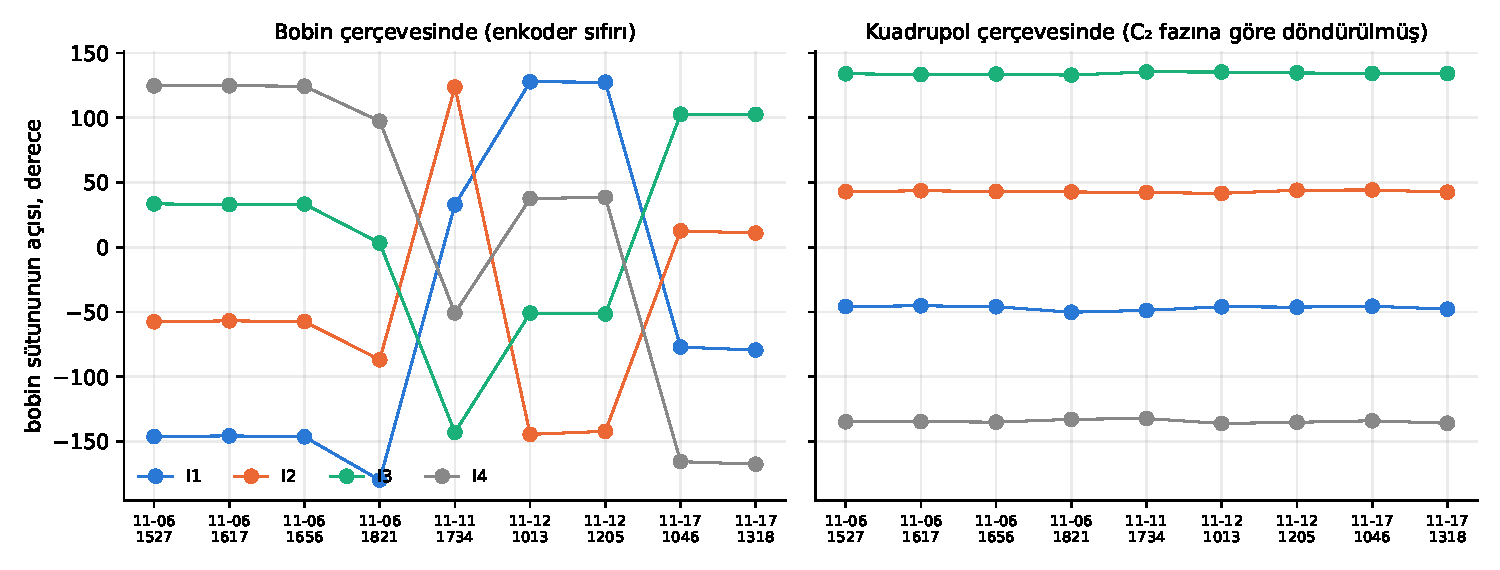
\includegraphics[width=\linewidth]{sekil1_matris.pdf}
\caption{Her bobinin merkezi ittiği yönün açısı. Solda enkoderin o günkü sıfırına göre (günden güne dağınık),
sağda kuadrupolün kendi eksenine göre (dokuz kalibrasyonda aynı).}
\label{fig:matris}
\end{figure}

\textbf{Yorum} \yor: matris mıknatısın geometrisine ait, bobinin ya da enkoderin nerede durduğuna değil. Değişen
tek şey dönen bobinin açı sıfırı. Bu yüzden kayıtlı matris başka bir oturumda, matrisin döndürülmesiyle
kullanılabilir. Yazılımda bu bir ``yön doğrulama'' adımı olarak yapıldı (Bölüm~\ref{sec:yazilim}).

\subsection{Enkoder artımlı: ``roll'' yerçekimine göre bir açı değil}
\label{sec:enkoder}

\kod{donen\_bobin/src/stator.cpp}'ye baktım: enkoder bir kuadratür (artımlı) enkoder, turda 3600 sayım, index
(Z) kanalı kullanılmıyor; sıfır noktası, program açıldığı ya da sayaç sıfırlandığı andaki konum \olc. Yazılımdaki
faz ofseti de bütün kayıtlarda 0. Sonuç olarak enkoder açısı oturumdan oturuma keyfi kayıyor. Arayüzde ``roll'' diye
gösterilen $\psi$ de 6--17 Kasım arasında $-82^\circ$ ile $+32^\circ$ arasında değişti (Tablo~\ref{tab:matris});
mıknatıs dönmedi, enkoderin sıfırı kaydı. Dolayısıyla bu sistem şimdiye kadar yerçekimine göre bir skew
ölçmedi \olc. Göstergelerin adlarını ``kuadrupol açısı (bobin sıfırına göre)'' ve ``a2/b2 (bobin çerçevesinde)''
yaptım; CSV sütun adları (\kod{roll\_mrad}, \kod{sq\_over\_g}) eski analizler bozulmasın diye değişmedi.

\textbf{Gradyen hesabı da etkilenmişti.} Gradyen, $C_2$'nin normal bileşeninden ($B_2/r_\text{ref}$) okunuyordu.
Normal bileşen enkoder çerçevesine bağlı olduğundan $B_2 = |C_2|\cos 2\psi$ (17 Kasım'da $\cos 2\psi = 0.45$, yani
gradyen hedefi gerçek değerin yalnızca \%45'iydi). $\psi$'deki 1~mrad'lik oynama gradyende, çalıştırmaya göre \%0.04 ile \%1.06 arasında (en kötüsü 6 Kasım akşamı ve
17 Kasım) sahte bir değişim gibi görünebiliyordu (tolerans \%0.1). Gradyen artık $|C_2|/r_\text{ref}$'ten hesaplanıyor
(\kod{gradyen\_kaynagi: genlik}).

\textbf{Yerçekimine göre skew nasıl ölçülür} \yor: dönen bobinin mili üzerine, bobinle aynı rijit gövdede bir
ivmeölçer takılır; motor birkaç açıda durdurulup ivmeölçerin okuması enkoder açısına karşı bir sinüse uydurulur, bu
yerçekiminin enkoder çerçevesindeki açısını verir. İvmeölçerle bobinin kuadrupol açı sıfırı arasındaki sabit
fark ise bobin sistemi kuadrupolün içinde uçtan uca çevrilerek bir kez ölçülür. Helmholtz bobiniyle referans alanı
üretmek önerilmedi: o yöntem bobinin dipol (n=1) açı sıfırını verir, kuadrupol (n=2) için gereken ise farklıdır;
iki iletkenin yarıçapı 0.1~mm farklıysa fark 2.5~mrad olur (hesap). Ayrıntı ve uygulama istemi
\kod{planlar/yercekimi\_referansi\_PROMPT.md}'dedir.

\subsection{18 Kasım donanım testleri}

\textbf{Test 1} (15:17, kayıtlı 17 Kasım kalibrasyonu, son akımlarla, 2~s'lik ölçüm) \olc.
Enkoder sıfırı 17 Kasım'dan beri kaymıştı: $\psi$ $+31.6^\circ$'den $+15.0^\circ$'ye geçmişti ve yazılım matrisi
$16.7^\circ$ döndürdü. Yön doğrulamanın H adımında ölçülen kayma öngörüden \%9 farklı, açı farkı $0.4^\circ$
çıktı: matris yeni oturumda geçerli. Kalibrasyon yinelenmediği için merkezleme yaklaşık bir dakikada bitti ama
5 yinelemede toleransa inemedi, merkez $(-11.0,\ +4.9)$~µm kaldı (Şekil~\ref{fig:testler}, sol). Dünün son
akımlarında merkez zaten yalnızca ~20~µm uzaktaydı: bobini kuadrupole sabitlemek işe yaramış.
10 dakikalık izlemede merkez, soğuk başlangıç nedeniyle y yönünde saatte yaklaşık 29~µm kaydı (günlük:
\kod{kayitlar/arayuz\_testi\_2026-11-18\_151722.log}). Bekçi testinde motor durdurulduktan 1 dakika sonra
uyarı çıktı.

\textbf{Test 2: tanı ölçümü} (15:31). Soru: 2~s'lik ölçümlerde merkez yinelemeler arasında neden 13--19~µm
sıçrıyor? 34 ölçüm alındı \olc:
\begin{itemize}
\item Aynı akımda 6 tekrar: $\sigma = 4.4$~µm (x), $2.6$~µm (y). Akım değiştikten hemen sonra ek bir gürültü yok.
\item $\pm 2.9$~mA'lik küçük adımlara tepki doğrusal: ölçülen $(-2.9,\ -15.5)$~µm, matrisin öngörüsü
$(-5.6,\ -16.8)$~µm; dört döngü arasında 1.2~µm tekrarlanabilir.
\item Aynı noktaya yukarıdan ve aşağıdan gelme farkı $(+6.1,\ +3.9)$~µm; sıfırdan geçip dönmenin etkisi
$(-1.8,\ +3.4)$~µm. İkisi de tek ölçümün gürültüsüne (4.4 ve 2.6~µm) göre yaklaşık iki sigma düzeyinde; anlamlı bir
histerezis \emph{kanıtlanmadı}, ama daha çok ölçümle ayrıca doğrulanabilir \yor.
\end{itemize}
Sonuç \yor: merkezleme her yinelemede tek bir 2~s'lik ölçümün gürültüsünü kovalıyordu; üstüne 10--20~s'lik yavaş
bir dalgalanma (5--10~µm) biniyor.

\textbf{Test 3} (15:37, ölçüm süresi 10~s) \olc. Merkezleme 5. yinelemede yakınsadı: $(+2.5,\ -1.4)$~µm,
122~s (Şekil~\ref{fig:testler}, sağ). Arka plan ölçümünün olduğu yinelemede merkez ~10~µm sıçradı; yakınsama
sınırda oldu.

\begin{figure}[h]
\centering
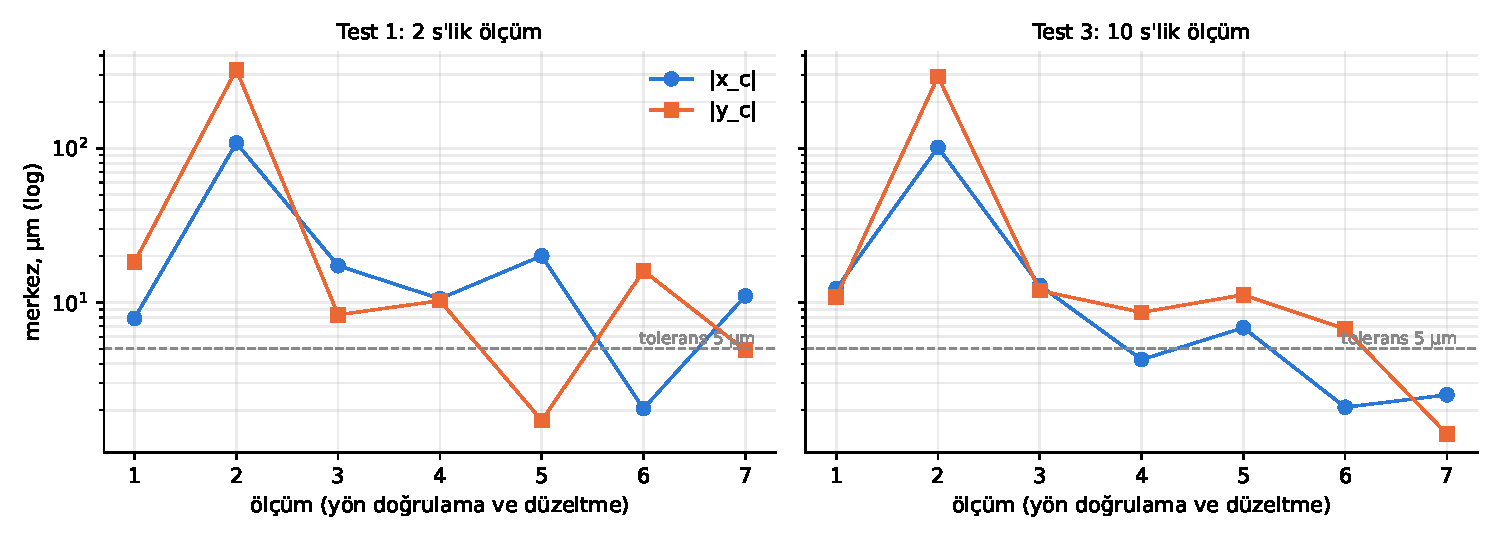
\includegraphics[width=\linewidth]{sekil2_testler.pdf}
\caption{Merkezleme yinelemelerinde mutlak merkez (log eksen). Solda 2~s'lik, sağda 10~s'lik ölçüm. İlk iki
nokta yön doğrulama, kalanlar düzeltme yinelemeleri.}
\label{fig:testler}
\end{figure}

\textbf{16:30 denemesi (sizin yaptığınız)} \olc. İlk deneme (\kod{calistirmalar/2026-11-18\_163037}) bir dakikadan
kısa sürdü ve durduruldu. İkincisi (\kod{...\_163232}) yeni bir kalibrasyon kurdu (9 nokta, yaklaşık 6 dakika);
nominal akımlardan başlayan ilk düzeltme ölçümünde merkez $(-900,\ +759)$~µm idi (nominal akımlarda merkez her
zaman ~1.1~mm uzaktadır). Bundan sonra ölçümler reddedilmeye başlandı ve motor durdu (aşağıda).

\subsection{``Okuma saati sıçraması'' eşiği}
\label{sec:sicrama}

Dönen bobin programı, bir ADC örneği kaybolursa bunu enkoder okumalarının düzenli ritminin bozulmasından
anlar: ``okuma saati sıçraması'' (örnek cinsinden) eşiği aşarsa ölçümü reddeder; üst üste üç ret motoru durdurur.
Eşik 0.6 idi. 16:30 oturumunda 33 ölçümün 17'si reddedildi ve üç ret art arda gelince motor durdu
(günlük: \kod{kayitlar/2026-11-18\_163044/gunluk.txt}) \olc. Bu, 17 Kasım'da ilk fark ettiğiniz ``motor
kendiliğinden durdu'' belirtisinin ikinci bir nedenidir; ilki yazılım hatasıydı (17 Kasım raporu).

Ham veriden (Tablo~\ref{tab:sicrama}, Şekil~\ref{fig:sicrama}) görülen \olc: sağlıklı veride de sıçrama
0.45--0.70 çıkıyor; 0.6 eşiği bu aralığın ortasında. 2~s'lik pencerede medyan 0.47 ve ölçümlerin \%4.6'sı eşiği
aşıyordu; 10~s'lik pencerede medyan yükseliyor (büyük olasılıkla kayan medyanın tepe-tepe değişimi pencereyle
birlikte büyüdüğünden \yor). Aynı ham verinin
2~s'lik dilimlerinde medyan 0.46, tamamında 0.61. Ayrıca oturumlar arasında fark var: 15:37 oturumu sessizdi
(medyan 0.50, hiç ret yok), 16:30 oturumu daha gürültülüydü (0.61). Büyük olasılıkla gerçek örnek kayıplarında değer 1.3--11
çıktı (üç oturumda motor başlatıldıktan hemen sonraki ilk ölçümde), yani sağlıklı gürültü ile kayıp arasında
0.70 ile yaklaşık 1.3 arasında bir boşluk var \yor.

\begin{table}[h]
\centering\small
\begin{tabular}{lrrrr}
\toprule
 & ölçüm & medyan & 0.6'yı aşan & 0.9'u aşan \\
\midrule
17 Kasım, sürekli ölçüm (2 s) & 10427 & 0.47 & \%4.6 & \%0.45 \\
18 Kasım 15:37 (test 3), 10 s & 9 & 0.50 & 0 / 9 & 0 / 9 \\
18 Kasım 16:30 (sizin deneme), 10 s & 33 & 0.61 & 17 / 33 & 1 / 33 \\

\bottomrule
\end{tabular}
\caption{Okuma saati sıçraması. 16:30 oturumunda 0.9'u aşan tek ölçüm, motor başlatıldıktan hemen sonraki ilk
ölçümdür (7.1).}
\label{tab:sicrama}
\end{table}

\begin{figure}[h]
\centering
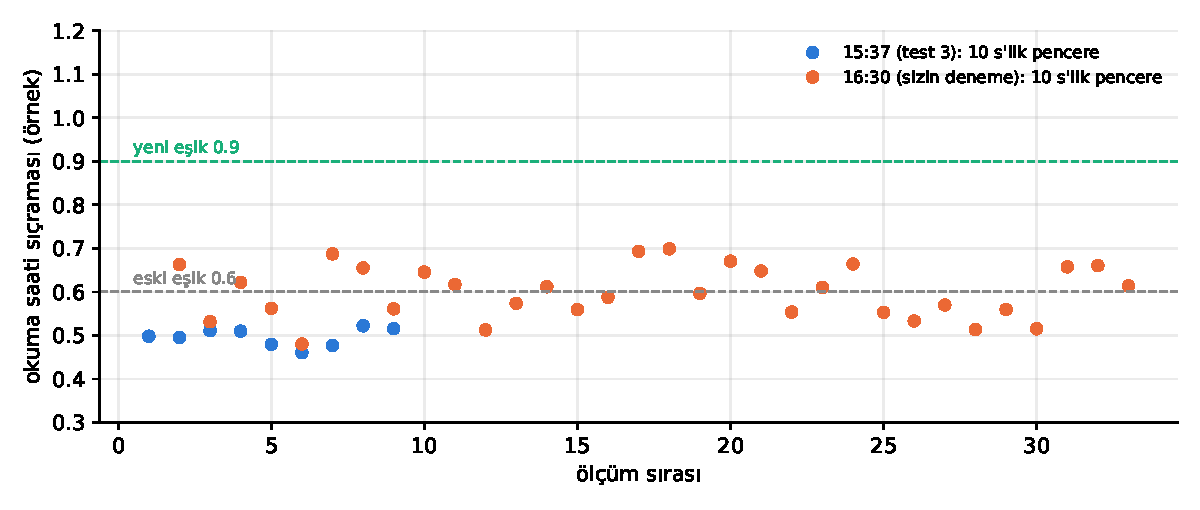
\includegraphics[width=0.8\linewidth]{sekil3_sicrama.pdf}
\caption{Her 10~s'lik ölçümün sıçrama değeri. Eşik 0.6'da 16:30 oturumunun yarısı reddedilir; 0.9'da yalnızca
ilk ölçüm kalır (7.1; grafiğin dışında).}
\label{fig:sicrama}
\end{figure}

\textbf{Yapılan:} eşiği \kod{donen\_bobin/merkezleme\_olcer.yaml}'da 0.6'dan 0.9'a çıkardım. Bu değişiklik
\textbf{donanımda denenmedi}. Kalan risk \hip: gerçek bir kayıp bazen 0.7--0.9 arasında bir değer verirse
(örnek sayım penceresinin kenarında olursa) artık geçebilir; elimizde yalnızca birkaç kayıp örneği var. Üst
üste üç retin motoru durdurması tasarım gereği; ama sağlıklı verinin eşiğe bu kadar yakın olduğu bir düzende bu
davranış tekrar sorun çıkarabilir (Bölüm~\ref{sec:acik}).

\subsection{Günler arası ve gün içi tekrarlanabilirlik}

6 Kasım öğleden sonrasından beri gerçek donanımda 9.5~A ile yapılan merkezlemeleri karşılaştırdım. Aynı gün
içindeki iki merkezleme birbirinden ``mA'' düzeyinde farklı akımlarda bitti (Tablo~\ref{tab:tekrar}). Günler
arasındaki fark büyük (yüzlerce mA), çünkü her gün bobin başka bir yerdeydi ve merkezleme mıknatısı bobin
eksenine göre ortalıyor \olc. En iyi durumda (6 Kasım, 40 dakika arayla) 22~µm'lik, 12 Kasım'da (iki saat arayla)
81~µm'lik fark var; bu, o günün 30--36~µm/saatlik merkez kaymasıyla uyumlu \yor.

\begin{table}[h]
\centering\small
\begin{tabular}{lllrr}
\toprule
gün & saat & akım farkı I1, I2, I3, I4 (mA) & ortak (mA) & merkezde (µm) \\
\midrule
06.11 & 16:17 → 16:56 & 5.4, 0.4, $-$4.7, 0.3 & 0.3 & 22 \\
12.11 & 10:13 → 12:05 & $-$10.8, 13.5, 4.0, $-$20.2 & $-$3.4 & 81 \\
17.11 & 10:46 → 13:18 & 30.4, 19.7, 8.8, 19.6 & 19.6 & 42 \\

\bottomrule
\end{tabular}
\caption{Aynı gün içindeki iki merkezlemenin son akımları arasındaki fark ve bunun o günün matrisiyle merkezdeki
karşılığı. ``Ortak'': dört akımın ortalama farkı (gradyeni korumak için birlikte kayar).}
\label{tab:tekrar}
\end{table}

\section{Yazılımda yapılanlar}
\label{sec:yazilim}

Bütün değişiklikler testleriyle birliktedir. Ayrıntılı gerekçeler commit mesajlarında ve README'dedir.

\textbf{Hata ve izleme:} boş ölçüm penceresi artık \kod{IndexError} yerine \kod{ValueError} verir (ölçüm atlanır,
motor durmaz); beklenmeyen hatanın yeri günlüğe yazılır; güç kaynağı akımının okunamaması günlüğe yazılır;
izlemede arka plan son 5 ölçümün ortalamasıdır; 60~s ölçüm gelmezse bekçi uyarır ve telefona Telegram bildirimi
gönderir; akımlar açıkken pencere kapatılırken sorulur.

\textbf{Merkezleme akışı:} toleransa ulaşmadan biten merkezleme ``TOLERANS DIŞINDA BİTTİ'' olarak gösterilir;
``olası yazım hatası'' uyarısı ``beklenenden sapma'' oldu (ve öngörünün bir önceki ölçümün akımlarına göre
hesaplanması gerekirken yanlış hesaplandığı hata düzeltildi: önceki sürümde her büyük adım uyarı veriyordu);
``Mevcut akımlarla yeniden düzelt'' düğmesi (akımlar sıfırlanmadan ve kalibrasyon yinelenmeden); arka plan her 3
noktada bir alınır (önceden her noktada; her arka planda mıknatıs soğuyordu); şüpheli kalibrasyon uyarısı kalıcı
görünür; aynı saniyede başlayan iki çalıştırma aynı klasöre yazmaz.

\textbf{Kayıtlı kalibrasyon:} kalibrasyon dosyası $\psi$'yi saklar (eski dosyalar için \kod{olcumler.csv}'den
tamamlanır); ayar panelinde ``Kalibrasyon'' seçimi ve ``son akımlardan başla''; yön doğrulama: iki ölçüm
(başlangıç akımları ve küçük bir H adımı), matris $\psi$ farkı kadar döndürülür, 180° belirsizliği H adımındaki
kaymayla çözülür, ölçülen ile öngörülen kayma $\pm15^\circ$/oran 0.7--1.4 dışındaysa akış durur ve yeni kalibrasyon
önerir.

\textbf{Varsayılan ayarlar (18 Kasım):} ölçüm süresi 2~s $\to$ 10~s, en fazla yineleme 5 $\to$ 8, dönen bobinden veri
bekleme zaman aşımı 30~s $\to$ 60~s, izleme kayıt aralığı 10~s $\to$ 30~s, arka plan her 3 noktada, sıçrama eşiği
0.6 $\to$ 0.9.

\textbf{Arayüz (\kod{arayuz-duzen} dalında):} her sekmede görünen alt durum çubuğu (kip, dönen bobin, akımlar,
çalıştırma); Merkezleme sekmesi: başlamadan önce ortada dar bir ``Yeni merkezleme'' kartı, çalışırken başlık
kartı (adım, ilerleme çubuğu, sonraki eylem), büyük x\_c / y\_c / g göstergeleri (tolerans içinde yeşil), merkezin
seyri grafiği, katlanır ayrıntılar; Kararlılık sekmesi: süre, ortalama $\pm\ \sigma$, kayma ve ölçüm akışı
göstergeleri; yeni Ayarlar sekmesi (ölçüm süresi, yineleme sayısı, arka plan aralığı, kalibrasyon adımı, izleme
aralığı, bekçi süresi, Telegram bildirimi, tema; donanım ve güvenlik sınırları salt okunur; ``Kalıcı yap'' YAML
dosyasını yorumlarını koruyarak günceller). Ekran görüntüleri ekransız (offscreen) alındı, açık ve koyu temada
kontrol edildi.

\section{Düzeltmelerim (bu çalışma sırasında yaptığım yanlışlar)}

\begin{itemize}
\item 17 Kasım raporunun ilk sürümünde ``gradyendeki ilk artış güç kaynaklarından gelmiyor'' demiştim; kaynağın
okuduğu akım, akımı ayarladığı aynı iç ölçüm direncinden geldiği için bu çıkarım geçersizdi. Rapor v2'de
düzeltildi. Bobinlerin ısınmasını da ilk önce 25~K diye bildirmiştim, doğrusu ~22~K.
\item ``Uçtan uca çevirme'' yöntemini anlatırken enkoderin sıfırının sabit olduğunu varsaymıştım. Enkoder artımlı;
bu varsayım yanlıştı (Bölüm~\ref{sec:enkoder}).
\item Arayüzdeki ``roll''un yerçekimine göre skew olduğunu varsayıyordum. Değildi.
\item Ölçüm süresini 10~s yaparken bunun saat sıçraması denetimine etkisini kontrol etmedim; 16:30'da motor
durdu (Bölüm~\ref{sec:sicrama}).
\item Tanı testi sonucunu ilk özetimde ``histerezis yok'' diye yazdım. Doğrusu: anlamlı histerezis
\emph{kanıtlanmadı}; fark iki sigma düzeyinde.
\end{itemize}

\section{Açık işler ve önerilen sıra}
\label{sec:acik}

Ayrıntılı liste \kod{planlar/YAPILACAKLAR.md}'dedir. Önerilen sıra:

\begin{enumerate}
\item \textbf{Bir sonraki donanım oturumunda önce kısa bir merkezleme denemesi} (\kod{main}, yeni eşik).
Günlükte ``Ölçüm reddedildi'' satırlarını sayın; çoksa eşik ve ölçüm süresi birlikte gözden geçirilmeli.
\item \textbf{Üst üste üç retin motoru durdurması.} Sağlıklı gürültü eşiğe yakınken bu davranış ölçümü kesiyor.
Önerim: motoru durdurmak yerine uyarı vermek ve ölçümü yeniden denemek, motoru yalnızca ağır bir bozulmada
(ör. artık oranı) durdurmak.
\item \textbf{Yeni arayüzü gerçek ekranda görüp birleştirmek.} Küçük ekranda taşma ve yazı boyutları
bakılmadı.
\item \textbf{Isınmanın kaynağını ayırmak:} bobinlere sıcaklık sensörü ve bir devrede bağımsız akım ölçümü (hassas
şönt ve multimetre ya da DCCT). 17 Kasım'da soğuk başlangıçta merkez 22~µm, kuadrupol açısı 0.55~mrad kaydı;
mıknatıstan mı güç kaynaklarından mı geldiği ayrılamadı.
\item \textbf{Yerçekimi referansı} (ivmeölçer takılınca): \kod{planlar/yercekimi\_referansi\_PROMPT.md}.
\item \textbf{``Şüpheli'' kalibrasyon denetimlerini kuadrupol çerçevesinde yapmak.} Dokuz kalibrasyonun yedisi
``şüpheli'' işaretli; nedenlerin (``H modu y\_c'yi etkiliyor, x\_c bekleniyordu'' gibi) çoğu muhtemelen eksen
yönünün enkoder sıfırına bağlı olmasından geliyor \hip.
\item \textbf{Üç ayrı çalıştırma yolunu (\kod{./merkezle}, \kod{./merkezle otomatik}, \kod{uzun\_kararlilik.py})
tek çekirdekte birleştirmek.} Düzeltmeler birine yapılınca ötekilerde eksik kalıyor.
\item \textbf{Uzak depoya göndermek:} \kod{git push origin main --tags} (isteğe bağlı; şimdilik gönderilmedi).
\end{enumerate}

\end{document}
